%\newpage

\subsection{Making Pycket an Independent Racket Implementation}
\label{subsec:pycket}

Pycket is first designed in 2014 as a high-performance JIT compiler
for Racket, generated using the RPython meta-tracing framework
\cite{bolz14-racket}. The language interpreter is based on the CEK
abstract machine and has the state $\langle e, \rho, \kappa \rangle$ ($e$ : control
(program AST), $\rho$ : environment, $\kappa$ : continuation)
\cite{felleisen87}. \figref{fig:cek} shows the transition rules and
how the CEK-loop is implemented in Pycket. The interpreter loop
continuously reduces the CEK triple until an empty continuation is
reached, which triggers a \emph{Done} exception that returns the
results.

\begin{figure}[h!]
  \small
\begin{align*}
e &::= x \mid \lambda x.\, e \mid e \; e\\
\kappa &::= [] \mid \mathsf{arg}(e,\rho){::}\kappa \mid \mathsf{fun}(v,\rho){::}\kappa
\end{align*}
\begin{align*}
\langle x, \rho, \kappa \rangle & \longmapsto
    \langle \rho(x), \rho, \kappa \rangle \\
\langle (e_1 \; e_2), \rho, \kappa \rangle & \longmapsto
    \langle e_1, \rho, \mathsf{arg}(e_2, \rho){::}\kappa \rangle \\
\langle v, \rho, \mathsf{arg}(e,\rho'){::}\kappa \rangle & \longmapsto
    \langle e, \rho', \mathsf{fun}(v,\rho){::}\kappa \rangle \\
\langle v, \rho, \mathsf{fun}(\lambda x. \, e, \rho'){::}\kappa \rangle & \longmapsto
    \langle e, \rho'[x\mapsto v], \kappa \rangle
\end{align*}
\begin{lstlisting}[mathescape]
                                    try:
                                      while True:
                                        ast, env, cont = ast.interpret(env, cont)
                                    except Done, e:
                                      return e.values
\end{lstlisting}
\caption{The CEK Machine transitions and the loop in Pycket. Figure taken from \cite{pycket15}.}
\label{fig:cek}
\end{figure}

In its original design, Pycket relies on the Racket executable to read
and expand a given module into a fully-expanded program
\cite{samth:11}. As shown in \figref{fig:old-pycket}, Pycket runs the
Racket's expander on a given module to fully expand the program, and
then generates AST for it and evaluates it within the interpreter
loop \cite{pycket15}.

\begin{figure}[h!]
  \centering
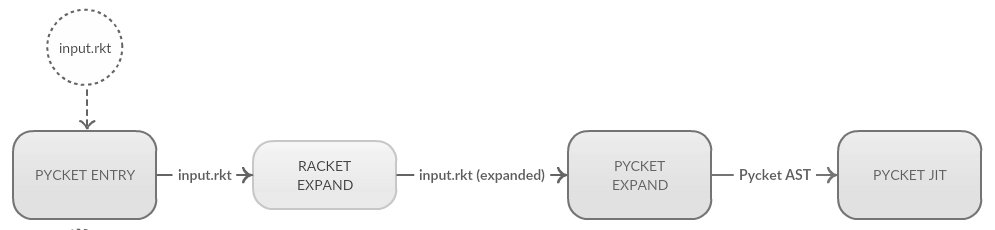
\includegraphics[scale=0.3]{img/old-pycket-grayscale}
\caption{Pycket used to run Racket's expander to fully expand a given module before running it.}
\label{fig:old-pycket}
\end{figure}


\begin{itemize}
  \item it was very fast, but relying on Racket binary to read and expand required modules
\item it used to be limited
\item we turned it into a full independent implementation using linklets
\end{itemize}


optimizations like common subexpression elimination, copy propogation, constant folding etc (cite Loop-aware optimizaitons....)

inlining comes for free from tracing (cite Hotpath VM)

loop invariant code motion (cite Loop-aware ....)

malloc-removal (cite Allocation removal ...)


- Here's how we can turn Pycket into a full Racket VM using linklets.

- Implementing linklets on CEK

- Bootstrap linklets

- Primitives

- Run-time support, exceptions, cont marks etc
